\documentclass[12pt]{article}
\usepackage[utf8]{inputenc}
\usepackage{float}
\usepackage{amsmath}

\usepackage[hmargin=3cm,vmargin=6.0cm]{geometry}
%\topmargin=0cm
\topmargin=-2cm
\addtolength{\textheight}{6.5cm}
\addtolength{\textwidth}{2.0cm}
%\setlength{\leftmargin}{-5cm}
\setlength{\oddsidemargin}{0.0cm}
\setlength{\evensidemargin}{0.0cm}

%misc libraries goes here

\usepackage{tikz}

\begin{document}

\section*{Student Information } 
%Write your full name and id number between the colon and newline
%Put one empty space character after colon and before newline
Full Name : Murat Bolu \\
Id Number : 2521300 \\

% Write your answers below the section tags
\section*{Answer 1}

\subsection*{a)}

\begin{itemize}
\item Since both $T_A$ and $T_B$ are uniformly distributed, their probability density functions are $f_A = f_B = \frac{1}{100}$ with $b = 100$ and $a = 0$. Since they are independent, the joint density function is $f(t_A, t_B) = f_A \cdot f_B = \frac{1}{10,000}$.
\item The joint cumulative distribution function is $F(t_A, t_B) = \iint \frac{dx \cdot dy}{10,000} = \int \frac{x \cdot dy}{10,000} = \frac{x \cdot y}{10,000}$.
\end{itemize}

\subsection*{b)}

Let's draw a $100 \times 100$ square to illustrate the probabilites. Since the probability density function is a constant function, the simple area of a region over ten thousand would give us the probability of an event being inside the region.

\begin{center}
    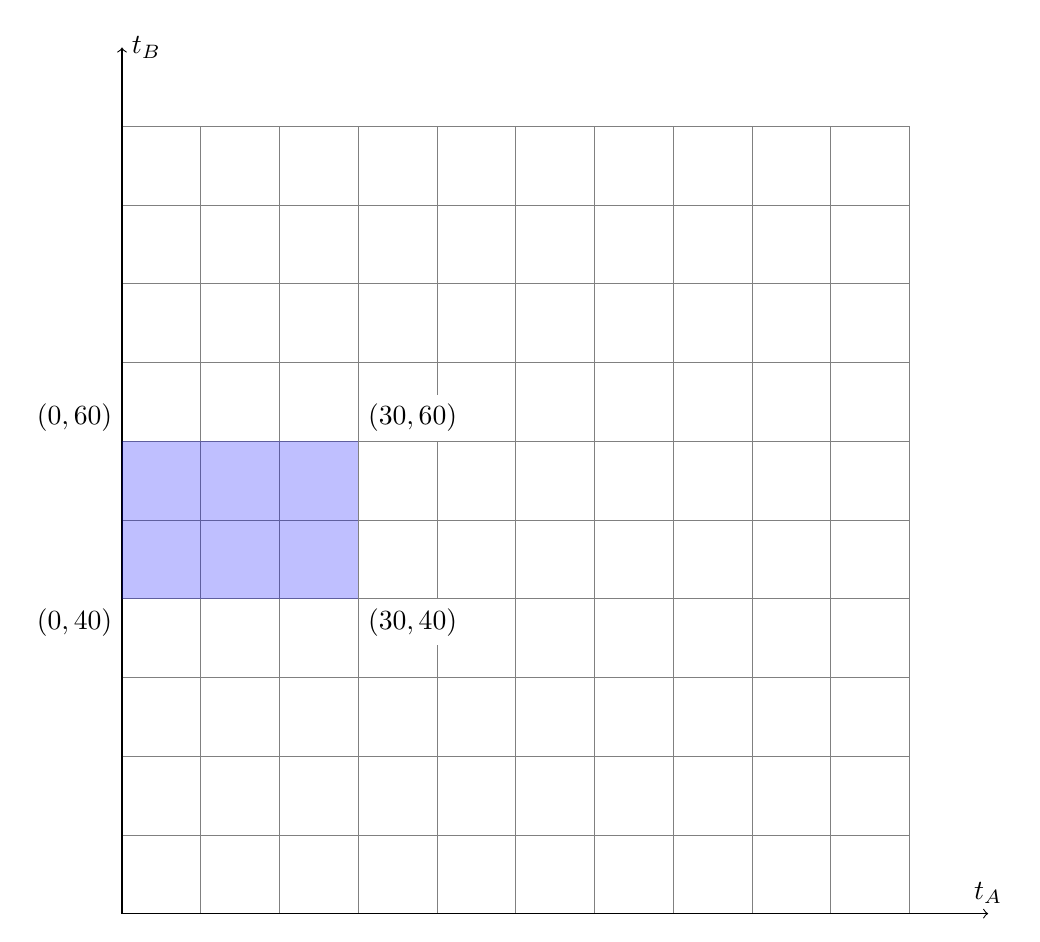
\begin{tikzpicture}
        \draw (0,0) rectangle (10,10);
        \draw [help lines] (0,0) grid (10,10);
        \draw [->] (0,0) -- (11,0) node [above] {$t_A$};
        \draw [->] (0,0) -- (0,11) node [right] {$t_B$};
        \fill [nearly transparent, blue] (0,4) -- (0, 6) -- (3,6) -- (3,4);
        \path (0,4) node [below left, fill=white]  {$(0, 40)$}
              (0,6) node [above left, fill=white]  {$(0, 60)$}
              (3,6) node [above right, fill=white] {$(30, 60)$}
              (3,4) node [below right, fill=white] {$(30, 40)$};
    \end{tikzpicture}
\end{center}


\subsection*{c)} 

\subsection*{d)} 


\section*{Answer 2}

\subsection*{a)} 

\subsection*{b)} 


\section*{Answer 3}


\section*{Answer 4}

\subsection*{a)} 

\subsection*{b)} 

\subsection*{c)} 

\end{document}